%Lab Report
\documentclass[12pt,titlepage, a4paper]{article}
 \usepackage[german]{babel}
 \usepackage[utf8]{inputenc}
 \usepackage{graphicx}
 \usepackage[table,usenames,dvipsnames,hyperref]{xcolor}
 \usepackage{multirow}
 \usepackage{caption}
 \usepackage{subcaption}
 \usepackage{amsmath}
 \usepackage{placeins} 
 \setlength{\parindent}{0in} 

\begin{document}

\title{Report\vspace{1cm}\\\textbf{Projektgruppe Kognitive Robotik}\vspace{5cm}}


\author{Münstermann,  Cedrick\\  Krombach, Nicola\\[1cm]
	Autonomous Intelligent Systems\\ \textsc{Universität Bonn}\\}



\maketitle



\section{Einleitung}

Im Rahmen der Projektgruppe Kognitive Robotik sollten in diesem Jahr die Aufgaben der European Robotics Challenges\footnote{http://www.euroc-project.eu/} bearbeitet werden.
Ziel dieser Challenge ist es, die Entwicklung von Lösungen für noch ungelöste Probleme in der Robotik anzutreiben.
In Form eines Wettbewerbs soll das Bewusstsein auf die Notwendigkeit der Entwicklung von Algorithmen für diese Probleme gelenkt, und Teams aus dem 
akademischen und industriellen Bereich ermuntert werden, sich zu beteiligen.
Die Aufgaben der European Robotics Challenges unterteilen sich dabei in drei Challenges, die wiederum verschiedene Unteraufgaben haben:

\begin{itemize}
 \item Challenge 1: Stationäre Manipulationsroboter in Kooperation mit Menschen \mbox{(Track 1 \& 2)}
 \item Challenge 2: Mobile Manipulationsroboter für die Logistik \mbox{(Track 1 \& 2)}
 \item Challenge 3: Flugroboter für industrielle Inspektion \mbox{(Track 1 \& 2)}
\end{itemize}

Unsere Gruppe befasste sich mit dem ersten Track der dritten Challenge, bei welchem die Lokalisierung eines Flugroboters (\textit{engl. Micro Aerial Vehicle, MAV}) und die 3D-Rekonstruktion 
der Umgebung im Vordergrund stand.
Für die Umgebungserkennung ist der in der Challenge eingesetzte Flugroboter mit einem Inertialsensor (\textit{engl. inertial measurement unit, IMU}) in Verbindung mit einem Stereokamerasystem ausgestattet. 


Autonome Flugroboter eignen sich aufgrund ihres flexiblen Aufbaus und der Möglichkeit schwer zugängliche Objekte anzufliegen, besonders für die Inspektion und Überwachung von sehr großen industriellen
Anlagen oder Infrastrukturen. Dabei sollen sie autonom agieren, sodass auf die Abhängigkeit von einem Piloten verzichtet werden kann.
Auch für die Inspektion von gefährlichen Umgebungen eignet sich ein autonomer Flugroboter.
Im folgenden werden die Aufgaben und entsprechenden Lösungsansätze von Track 1 vorgestellt.





\section{Aufgabenstellung} 
Der erste Track von Challenge 3 befasst sich vorrangig mit der Verarbeitung von visuellen Informationen und Geschwindigkeiten, welche die IMU liefert, um die Pose des MAV zu schätzen
und schließlich eine Karte von der Umgebung aufzubauen. Beide Aufgaben, Lokalisierung und Kartierung, lassen sich unabhängig voneinander lösen.



\subsection{Task 1 - Visuelle Lokalisierung}
In der ersten Aufgabe ging es darum aus Stereobildern eine 6D-Pose zu schätzen. Dazu wurden realistische Datensätze mit unterschiedlichen Schwierigkeiten zur Verfügung gestellt.
Ausschließlich anhand dieser Datensätze sollte nun die Lokalisierung erfolgen. Für die Evaluation war sowohl die lokale Genauigkeit als auch die Echtzeitfähigkeit der Berechnung entscheidend.
Eine Übersicht der Evaluierungskriterien und Punkteverteilung findet sich im bereitgestellten technischem Annex\cite{eurocannex}.
Neben den Kamerabildern wurden zudem eine Kalibrierung des Stereokamerasystems und der IMU zur Verfügung gestellt. 
Für die Berechnung der visuellen Odometrie wurden zunächst zwei bereits in ROS verfügbare Verfahren installiert und getestet:\\
Das Paket Semi-direct Monocular Visual Odometry (SVO)\cite{EPFL-CONF-199740} und das Paket \mbox{LIBVISO2}-Paket \cite{Geiger11}.
In ersten Experimenten stellte sich das \mbox{LIBVISO2} für unsere Zwecke als besser geeignet heraus, und zudem erlaubt es die Verwendung von Stereokameras für die visuelle Odometrie, 
im Gegensatz zu SVO, welches ein monokulares Verfahren ist.
Als Kamerakalibrierung wurde die bereitgestellte Kalibrierung mittels Aprilboard verwendet. Da diese jedoch nicht in dem von \mbox{LIBVISO2} verwendeten OpenCV-Format war, wandelten wir es mit Hilfe von OpenCV
in ein konformes Format um.
Für die korrekte Darstellung der Pose in IMU-Koordinaten, rechneten wir die aus den Stereobildern gewonnene Pose, mittels einer statischen Transformation aus der Kalibrierung, von Kamerakoordinaten 
in IMU-Koordinaten um.
Die sich dadurch ergebende Transformationskette lautet:\\

$  map \rightarrow imu \rightarrow cam0 $\\

\begin{figure}[t]
 \centering
  \begin{subfigure}[b]{0.49\textwidth}
 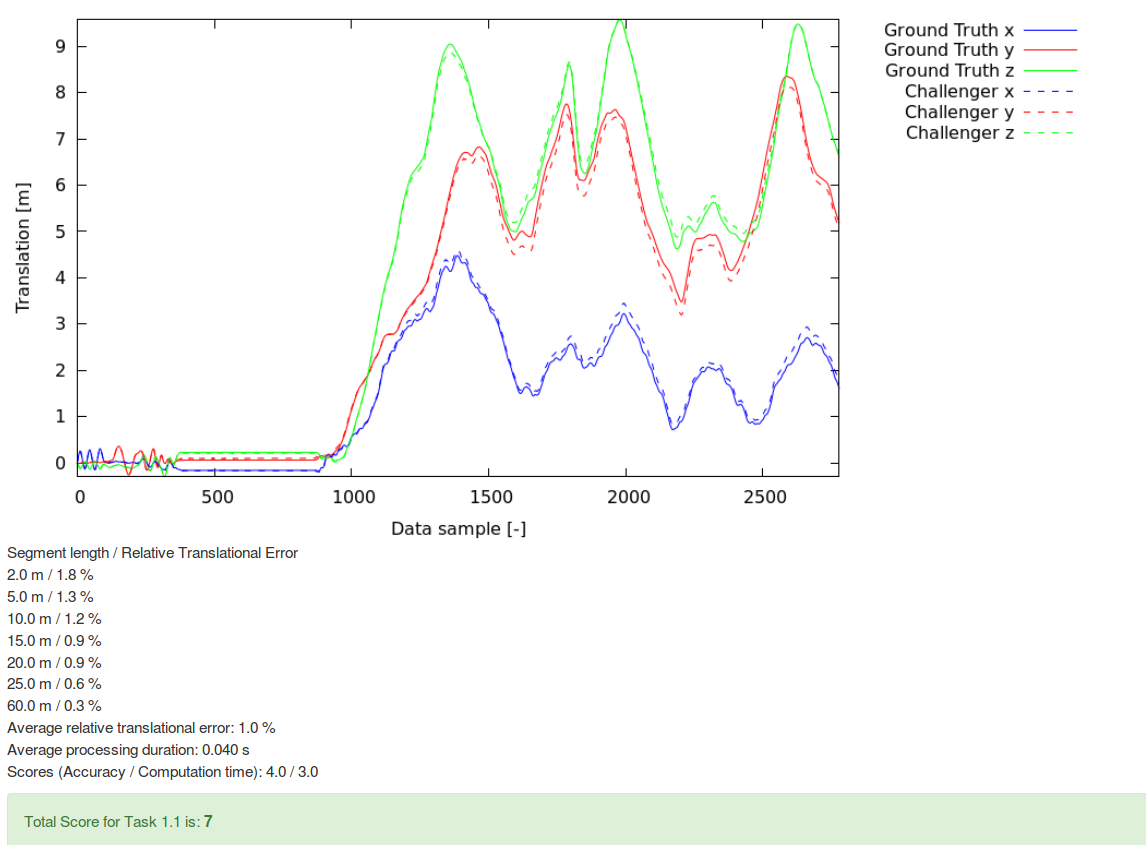
\includegraphics[width=\textwidth]{./Screens/t1_opt2_april.png}\caption{Task 1.1}\label{fig:evat1}  \end{subfigure}
  \begin{subfigure}[b]{0.49\textwidth}
 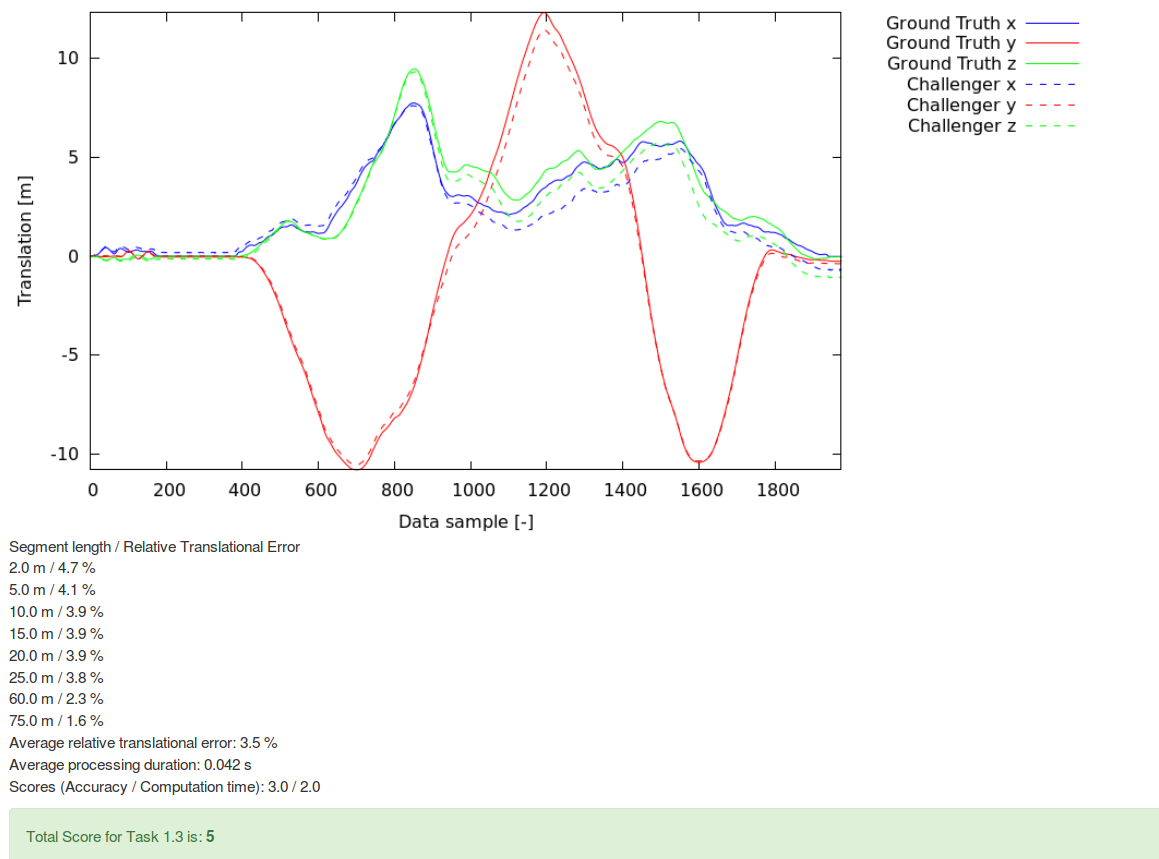
\includegraphics[width=\textwidth]{./Screens/t1_3.png}\caption{Task 1.3}\label{fig:evat3}
 \end{subfigure}
 \caption{Ergebnis der Online-Evaluation zu Task 1.1 und 1.3 mit 7 von 8 (bzw 5 von 8) möglichen Punkten} \label{fig:eva} 
\end{figure}\begin{figure}[h!]
 \centering
  \begin{subfigure}[b]{0.49\textwidth}
 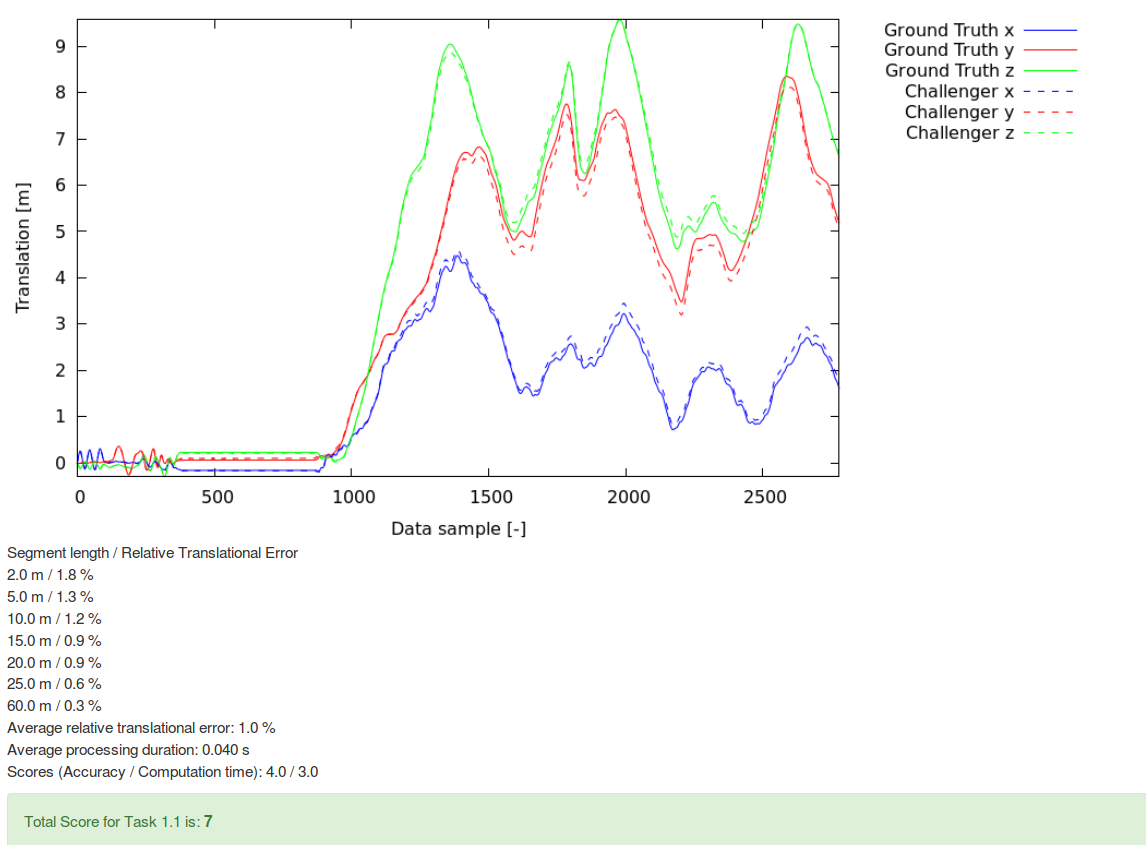
\includegraphics[width=\textwidth]{./Screens/t1_opt2_april.png}\caption{Task 1.1}\label{fig:evat1}  \end{subfigure}
  \begin{subfigure}[b]{0.49\textwidth}
 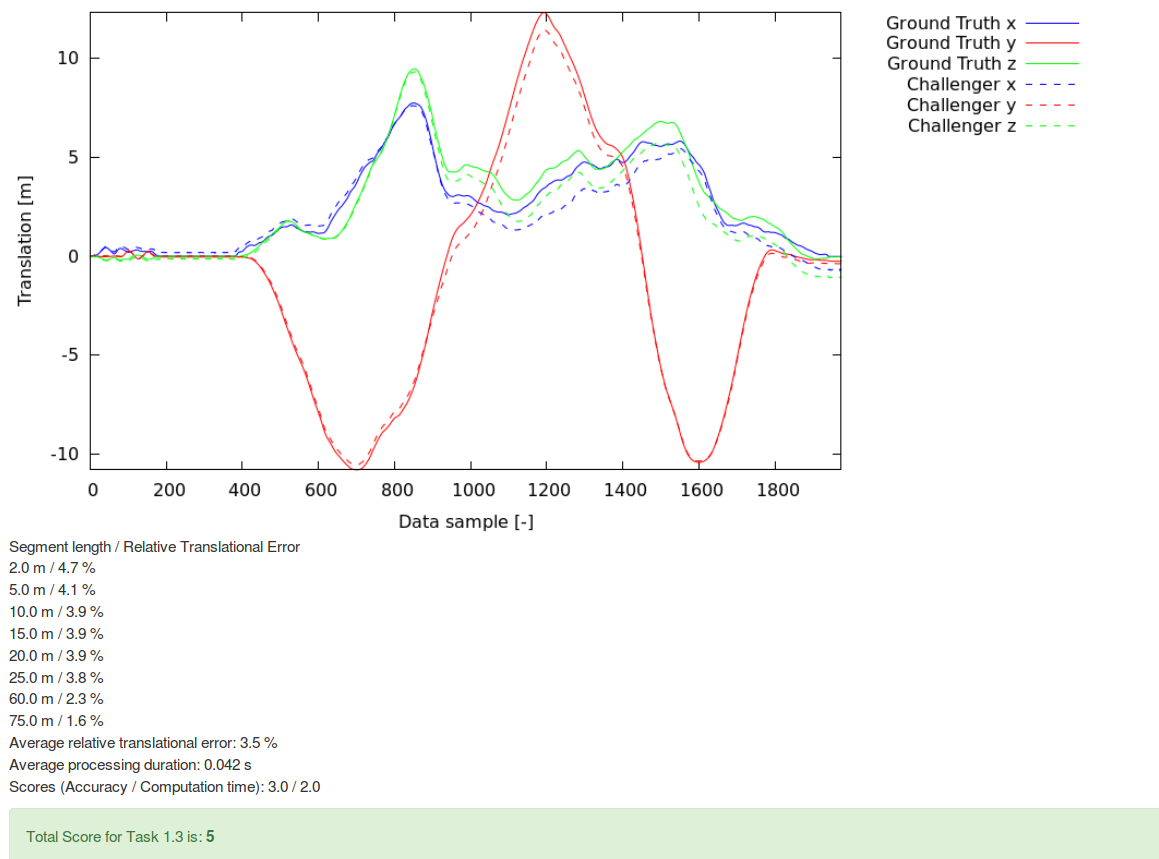
\includegraphics[width=\textwidth]{./Screens/t1_3.png}\caption{Task 1.3}\label{fig:evat3}
 \end{subfigure}
 \caption{Ergebnis der Online-Evaluation zu Task 1.1 und 1.3 mit 7 von 8 (bzw 5 von 8) möglichen Punkten} \label{fig:eva} 
\end{figure}

Da keine Groundtruth zur Verfügung gestellt wurde, konnte man letztlich nur über die Online-Evaluation herausfinden, wie genau die berechnete Pose ist und wie hoch der relative Fehler ist.
Mit den Default-Werten von \mbox{LIBVISO2} erhielten wir zu Beginn 4 Punkte bei der einfachsten Schwierigkeit. 
Davon 3 Punkte in der Genauigkeit mit einem mittleren relativen Translationsfehler von 2.6\% und 1 Punkt in der Laufzeit mit 105ms.
Die Laufzeit konnten wir mit dem Setzen des Compiler-Flags \textit{DCMAKE\_BUILD\_TYPE} auf \textit{Release} auf 39ms reduzieren, und erhielten so 3 Punkte in der Laufzeit.
Für die Erhöhung der Genauigkeit passten wir die Parameter von \mbox{LIBVISO2} an die unterschiedlichen Schwierigkeiten an. 
So erhöhten wir den Parameter match\_radius von 100 auf 200 und die RANSAC-Iterationen von 150 auf 160.
Damit konnten wir den Fehler von 2.6\% auf 1.0\% reduzieren, und erhalten damit volle Punktzahl in der Genauigkeit.
Ein Beispiel einer solchen Evaluation ist in Abbildung~\ref{fig:evat1} zu sehen. Dort schneiden wir in der Genauigkeit sehr gut ab, mit einem gemittelten relativen Translationsfehler 
von 1\% erhalten wir für die Genauigkeit volle Punktzahl. Auch in der Laufzeit sind wir mit 40ms verhältnismäßig gut. Für die volle Punktzahl benötigt man eine Laufzeit kleiner 20ms.
Auch in der zweiten Schwierigkeitsstufe erhalten wir mit 8 von 10 möglichen Punkten ein gutes Ergebnis für die berechnete Odometrie. In der schwierigsten Stufe hat die visuelle Odometrie
jedoch einige Probleme die korrekte Pose zu schätzen, was durch die schlechteren Belichtungsverhältnisse und merkmalsärmere Umgebung zu erlären ist.
Wie in Abbildung~\ref{fig:evat3} zu sehen, driften wir vor allem in x- und y-Richtung stark.


\begin{table}
\colorlet{tablerowcolor}{green!10.0} 
\centering
\begin{tabular}{c|c|c}
Task & Bewertungsintervall & Punkte\\
\hline
\multirow{5}{*}{1.1 Genauigkeit e} & e \textgreater 20\% & 0 \\
 & e \textless 20\% & 1\\  
  & e \textless 10\% & 2\\
   & e \textless 4\% & 3\\
 &\cellcolor{green!10.0} e \textless 2\% & \cellcolor{green!10.0}4\\
\hline
\multirow{5}{*}{1.1 Laufzeit t} & t \textgreater 200ms & 0 \\
 & t \textless 200ms & 1\\  
  & t \textless 100ms & 2\\
  & \cellcolor{green!10.0}t \textless 40ms &\cellcolor{green!10.0} 3\\
 & t \textless 20ms & 4\\
\hline
\end{tabular}\\
\vspace{10mm}
\caption{Bewertungssystem von EuRoC für Challenge 3 Task 1.1, grün hervorgehoben sind die erziehlten Ergebnisse}
\label{table:scoringt1}
\end{table}

\FloatBarrier
			
\subsection{Task 2 - Kartierung}
In der zweiten Teilaufgabe, der dritten Challenge, sollte eine 3D-Karte mit Hilfe des octomap-Frameworks von Hornung \cite{hornung13auro} aus Stereobildpaaren und einer jeweils zugehörigen 6D-Pose erstellt werden. Die generierte Karte konnte online überprüft werden. Bewertet wurde anhand des Matthew-Correlation-Coefficient und der Laufzeit (Siehe Tabelle 2). Der Matthew-Correlation-Coefficient nutz das Verhätnis zwischen den als falsch-frei, falsch-belegt, echt-frei und echt-belegt klassifizierten Voxeln.\\
$MCC = \frac{TP \times TN - FP \times FN}{\sqrt{(TP+FP)(TP+FN)(TN+FP)(TN+FN)}}$\\
Wir wollten dem octomap-Framework dichte Punktwolken als Eingabe übergeben, deshlab entschieden wir uns für LIBELAS von Geiger \cite{Geiger2010ACCV}. Die Installation von LIBELAS erwies sich aufwendiger als angenommen, da es ROS-Hydro und catkin noch nicht direkt unterstützt. Damit LIBELAS unsere Stereobilder gut verarbeiten konnte, mussten diese zunächst noch rektifiziert werden. Mit Hilfe von OpenCV und der gegebenen Kameakalibrierung, die wir schon im ersten Teil in ein OpenCV-konformes Format umgewandelt hatten, war dieser Schritt schnell getan. Was noch fehlte war eine Spezifizierung der Transformationskette vom map-Koordinatensystem in das Kamera-Koordinatensystem. Die Betrachtung der Posen-Nachricht, die der Server bereitstellte, führte zu dem Schluss, dass die Pose im IMU-Koordinaten war. Zusätzlich zu den rektifizierten Bildern und der Pose musste nun also auch noch ein Transformation vom map-Koordinatensystem in das IMU-Koordiantensystem verfügbar gemacht werden. Die statische Transformation von dem IMU-System in das Kamera-System war schon aus der ersten Teilaufgabe von Track 1 bekannt. Da nun alle Anforderungen der beiden benutzen Frameworks erfüllt waren, konnte die erste Karte erstellt werden. Diese sah auch schon recht gut aus und stimmte größtenteils mit der von uns handgezeichneten Karte überein. Leider gab es nur wenig Punkte für die Karte. Zwei Punkte für die Akkuratesse und Null für die Laufzeit. Durch das Überspringen einiger Bilder, konnte die Laufzeit einfach reduziert werden. Das Problem bei der Akkuratesse war, das wir viele falsch-belegte Zellen hatten (ca. 27000). Dies führte zu einem Ungleichgewicht im Korrelations-Koeffizienten. 

Zunächst war es jedoch wichtiger, die Genauigkeit der Karte zu verbessern. Die generierte Voxel-Karte hatte relativ dicke Wände und wir waren uns unsicher, inwiefern dies mit in die Bewertung genommen wurde. Als erstes sollten die Wände dünner werden. Bei Betrachtung der Punktwolke fiel auf, dass an den Rändern keilförmige Falschmessungen in den umliegenden Raum ragten. Ein erster Lösungsansatz bestand darin, einen Filter zu implementieren, der über das Disparitätsbild mit einem Box-Kernel lief und, im jeweils betrachten Ausschnitt, nach dem Minimum und dem Maximum suchte. Falls die Differenz der Beiden über einem anpassbaren Schwellwert lag, wurde der Ausschnitt verwofen. Im Falle von LIBELAS beduete dies, den Ausschnitt auf -10 zu setzen. Leider führte dieses Vorgehen nicht zur Eleminierung der Falschmessungen (siehe Abbildung 2).

\begin{figure}[h!]
	\centering
	\begin{subfigure}[h]{0.45\textwidth}
		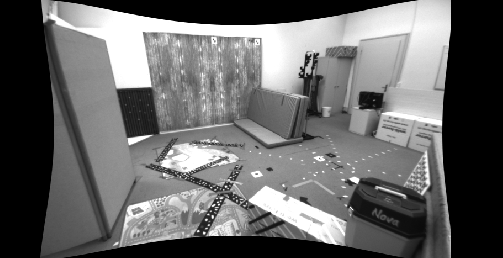
\includegraphics[width=\textwidth]{./jumpEdge/camera.png}
		\caption{Szene}
	\end{subfigure}\\
	\begin{subfigure}[h]{0.45\textwidth}
		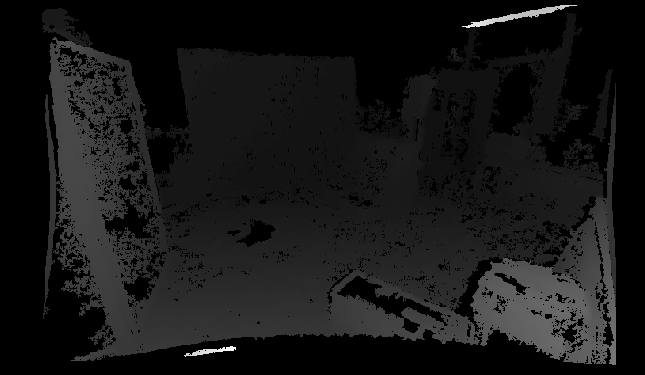
\includegraphics[width=\textwidth]{./jumpEdge/je_off_disparity.png}
		\caption{min-max aus}
	\end{subfigure}
	\begin{subfigure}[h]{0.45\textwidth}
		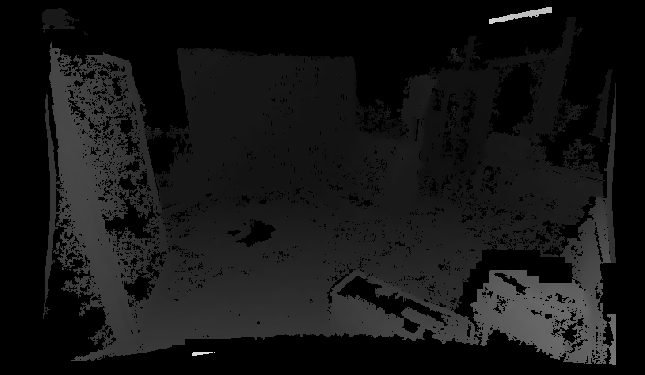
\includegraphics[width=\textwidth]{./jumpEdge/je_on_disparity.png}
		\caption{min-max an}
	\end{subfigure}
	\begin{subfigure}[h]{0.45\textwidth}
		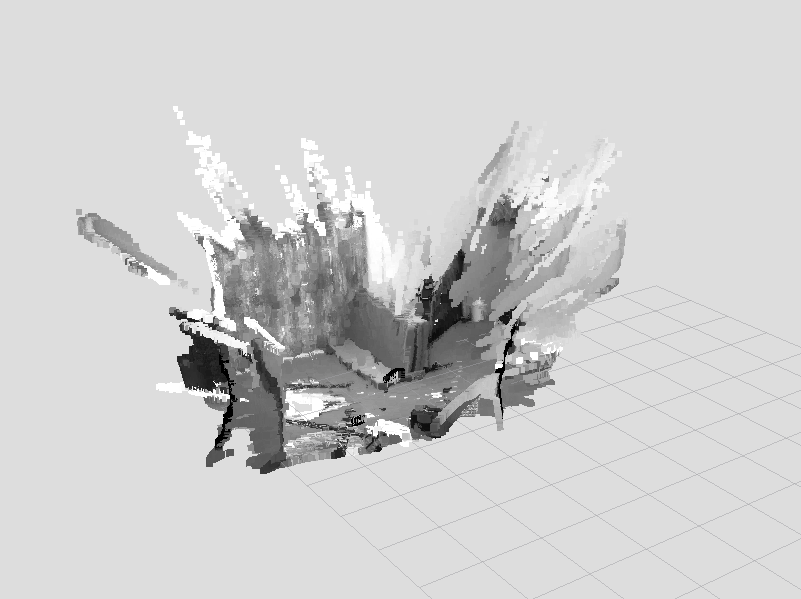
\includegraphics[width=\textwidth]{./jumpEdge/je_off_pointcloud.png}
		\caption{min-max aus}
	\end{subfigure}
	\begin{subfigure}[h]{0.45\textwidth}
		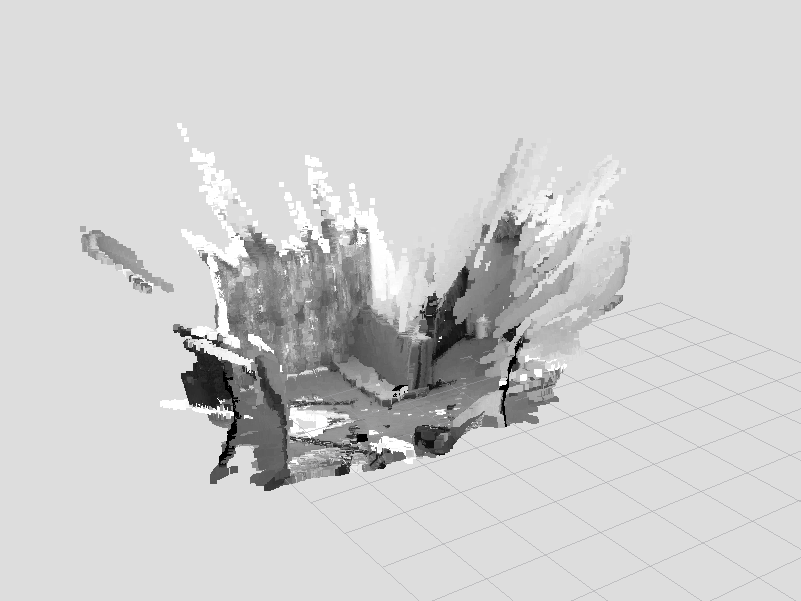
\includegraphics[width=\textwidth]{./jumpEdge/je_on_pointcloud.png}
		\caption{min-max an}
	\end{subfigure}	
 \caption{Pipeline}
\end{figure}

Eine weitere Idee, um die Wände zu verdünnen und Falschmessungen zu eliminieren, war die generierte Karte auszudünnen (Pruning), nachdem der Schwellwert für die Belegung (occcupancy-threshold) erhöht wurde. Dies führte dann auch zu einer sichtbaren Veränderung in der Karte. Die Wände wurden etwas dünner und einige, ehemals als belegt klassifizierte, Voxel wurden zu unbekannt oder frei. Auf die finale Bewertung der Karte, hatte das aber nur minimale Auswirkungen. Auch Parameteranpassungen in LIBELAS, vorallem des Parameters, der die Interplation über die Lücken im Disparitätsbild bestimmte, hatten wenig sichtbare Auswirkungen auf das Resultat. Die Interpolation führte dazu, dass im Disparitätsbild sehr harte Übergänge in den interpolierten Bereichen auftraten. Um dies zu verhindern filterten wir das Original-Disparitätsbild mit einem Gauss-Filter, um glatte Ränder rundum die Lücken zu bekommen. Dannach ließen wir LIEBELAS interpolieren und kopierten, die weich interpolierten Lücken zurück in das Original-Disparitätsbild. So blieben die interessanten Merkmale erhalten und es wurden keine harten Übergänge durch die Interpolation erzeugt. Dieses Vorgehen funktionierte aber nicht so ohne Weiteres, da der Gauss-Filter von OpenCV den, von LIBELAS als nicht klassifizierten, Bereich mit in die Berechnung einbezog. Deshalb wurde die Idee wieder verworfen. Wir beschlossen ganz auf die Interpolation über die Lücken zu verzichten.

Wir entschlossen uns eine e-mail an den Support zu schreiben, um nachzufragen wo genau unser Problem lag.
Zwischenzeitlich hatten wir auch die Vermutung, dass unsere generierte Karte in einem falschen Koordinatensystem lag und es deshalb zu der mittelmäßigen Bewertung kam.
Wie sich dann durch die Antwort des Supports herausstellte, waren jedoch weder die dicken Wände, noch das Koordinatensystem unser Problem. Das Bewertungssystem wertete auch als unbekannt klassifizierte Voxel, die frei sein sollten, als falsch-belegt. Unser Problem war, dass wir zu viele Unbekannte in der Nähe der Decke und den Wände hatten (siehe Abbildung 3).

\begin{table}
\colorlet{tablerowcolor}{green!10.0} 
\centering
\begin{tabular}{c|c|c}
Task & Bewertungsintervall & Punkte\\
\hline
\multirow{5}{210pt}{2.1 Fehler gemessen an Matthews Correlation Coefficient s} & 0 \textless s \textless 0.4 & 0 \\
 & 0.4 \textless  s \textless 0.6 & 1\\  
  & 0.6 \textless  s \textless 0.8 & 2\\
 & \cellcolor{green!10.0}0.8 \textless  s \textless 0.9 &\cellcolor{green!10.0} 3\\
 & 0.9 \textless  s \textless 1.0 & 4\\
\hline
\multirow{5}{210pt}{2.1 Laufzeit t} & t \textgreater $t_{max}$ & 0 \\
 & t \textless $t_{max}$ & 1\\  
  &\cellcolor{green!10.0} t \textless $0.5 t_{max}$ &\cellcolor{green!10.0} 2\\
  & t \textless $0.2 t_{max}$ & 3\\
 & t \textless $0.1 t_{max}$ & 4\\
\hline
\end{tabular}\\
\vspace{10mm}
\caption{Bewertungssystem von EuRoC für Challenge 3 Task 2.1, grün hervorgehoben sind die erziehlten Ergebnisse}
\label{table:scoringt2}
\end{table}

Die Idee war, den Freiraum immer dann zu expandieren, wenn ein als frei klassifizierter Voxel einen Nachbarn hatte, der unbekannt war. Aufgrund der Speicherung der Karte in einem Octree, sind Voxel, die unbekannt sind, nicht explizit in der Datenstruktur gespeichert. Die Expansion des Freiraums führte schließlich zu einer deutlichen Verbesserung in der Bewertung. Durch verschiedene Testläufe fanden wir heraus, dass die 4-malige Expansion des Freiraums zu dem besten Ergebnis führten. Noch besser wurde es wenn die fertige Karte vor der Expansion des Freiraums, noch mit einem leicht angepassten Belegungs-Schwellwert (von 0.7 auf 0.75) ausgedünnt wurde (siehe Abbildung 4). 

\begin{figure}[h!]
	\centering
	\begin{subfigure}[h]{0.45\textwidth}
		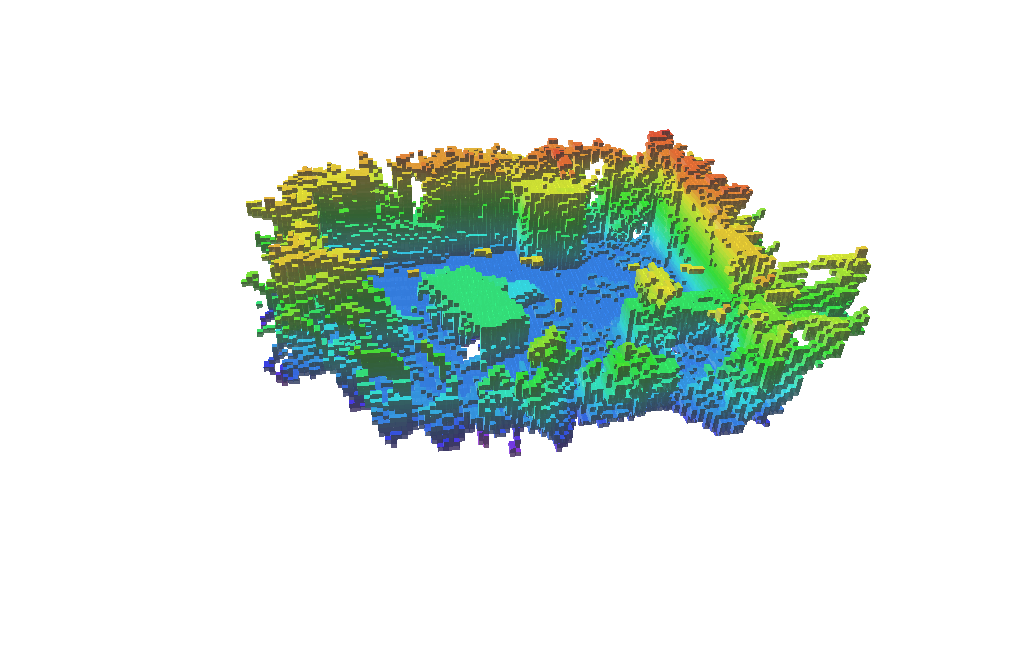
\includegraphics[width=\textwidth]{./maps/beforePrune.png}
		\caption{before pruning}
	\end{subfigure}
	\begin{subfigure}[h]{0.45\textwidth}
		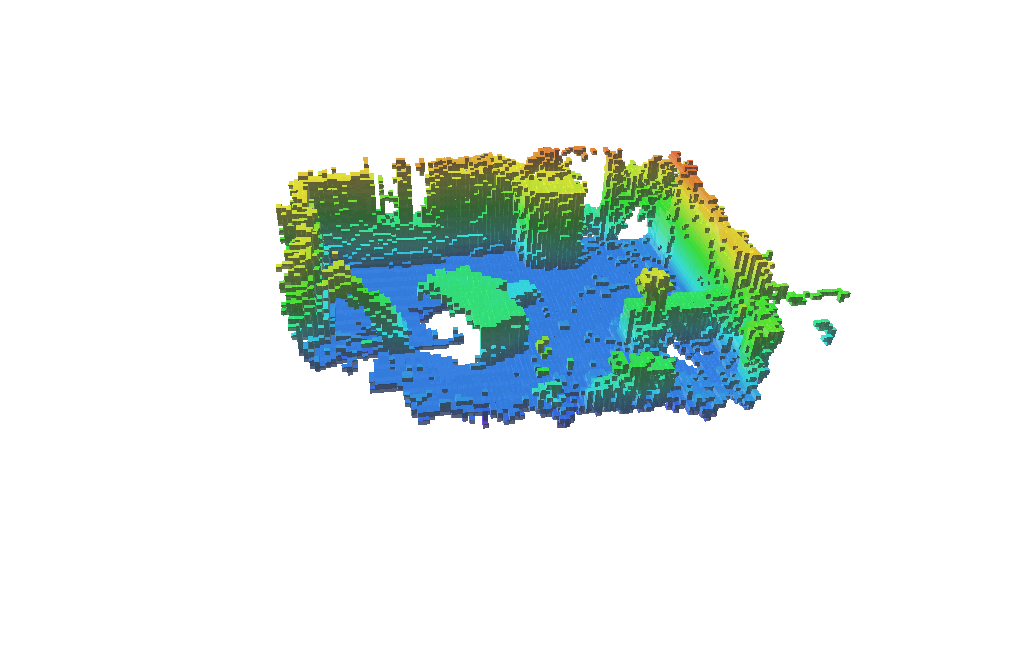
\includegraphics[width=\textwidth]{./maps/beforeMorph.png}
		\caption{after pruning}
	\end{subfigure}\\
	\begin{subfigure}[h]{0.45\textwidth}
		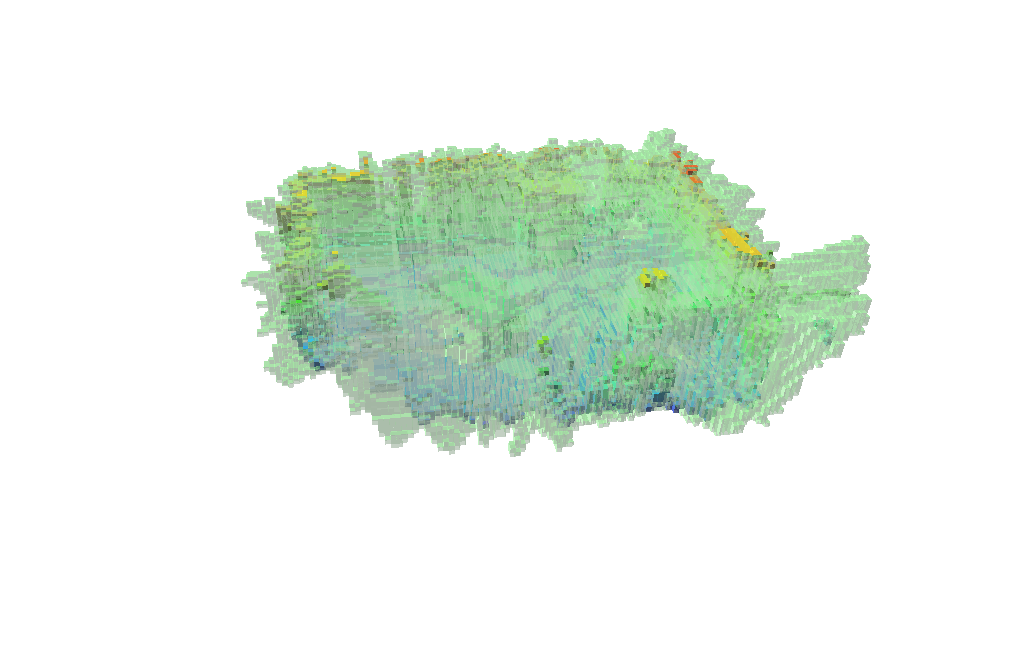
\includegraphics[width=\textwidth]{./maps/beforeMorph_free.png}
		\caption{before morphing with free space}
	\end{subfigure}
	\begin{subfigure}[h]{0.45\textwidth}
		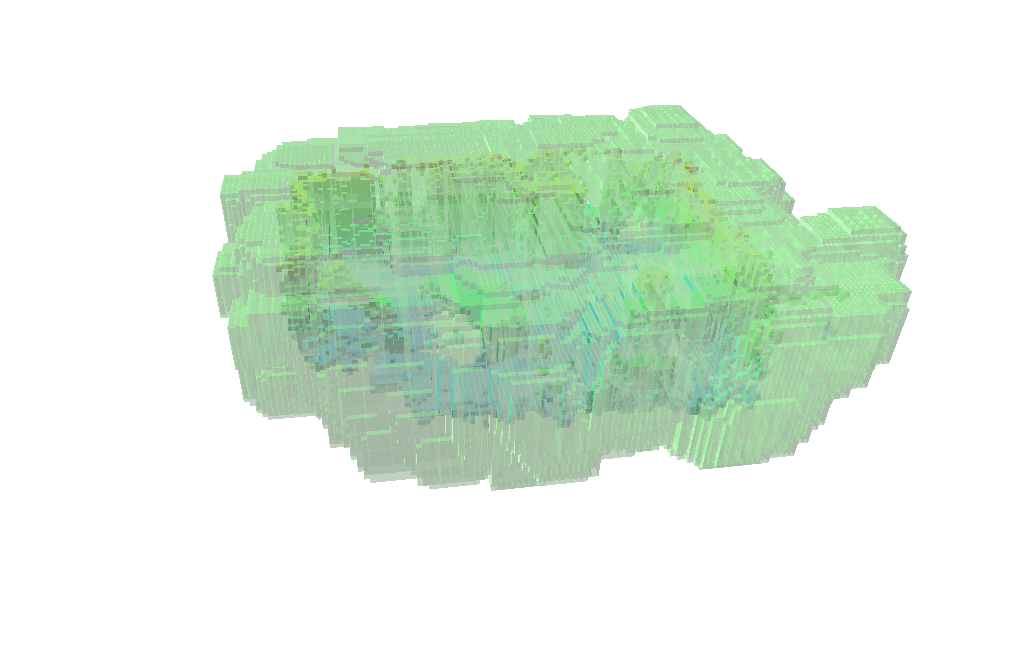
\includegraphics[width=\textwidth]{./maps/afterMorph_free.png}
		\caption{after morphing with free space}
	\end{subfigure}
 \caption{Pipeline}
\end{figure}

\begin{figure}[h!]
 \centering
 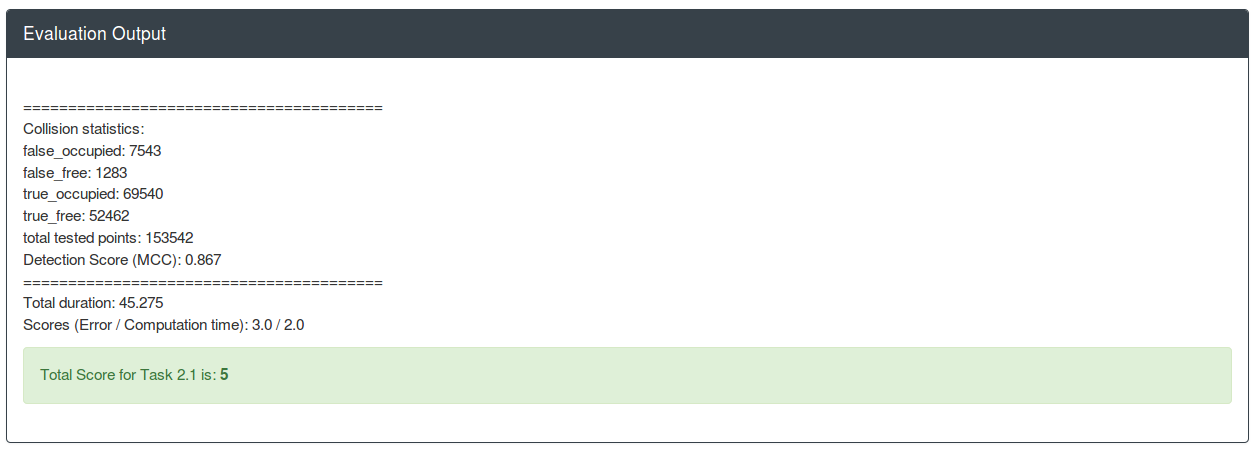
\includegraphics[width=0.5\textwidth]{./Screens/evaltask2.png}
 \caption{Resultat}
\end{figure}

\FloatBarrier

\section{Zusammenfassung}

-> Verbesserungsvorschläge:
Laufzeit ( aus ROS Overload verzichten)
IMU Informationen einrechnen

Es sind jedoch nach wie vor einige falsch-belegete Voxel übrig und als nächster Schritt wäre es möglich, belegete Voxel die weniger als 4 Nachbarn haben die belegt sind als frei zu klassifizieren.

\begin{table}
\colorlet{tablerowcolor}{green!10.0} 
\centering
\begin{tabular}{c|c|c}
\multicolumn{3}{c}{Visuelle Lokalisierung}\vspace{2mm}\\
Task 1.1 & Task 1.2 & Task 1.3\\
\hline\vspace{2mm}
7/8 & 8/10 & 6/8\\
\multicolumn{3}{c}{ }\\
\multicolumn{3}{c}{3D-Kartierung}\vspace{2mm}\\
Task 2.1 & Task 2.2 & Task 2.3\\
\hline\vspace{2mm}
5/8 & 6.5/10 & 5/8\\
\end{tabular}
\caption{Erziehlte Ergebnisse und maximale Punktzahl für Track 1}
\label{table:finalscore1}
\end{table}


\begin{table}
\colorlet{tablerowcolor}{green!10.0} 
\centering
\begin{tabular}{c|c|c|c}
Aufgabe & erziehlte Punkte & maximale Punkte & ???\\
\hline
Task 1 & 21 & 26 & 80.77\% \\
Task 2 & 16.5 & 26 & 63.46\% \\
\hline
\hline
 & & \\
Total & 37.5 & 52 & 72.12\%\\
\end{tabular}
\caption{Übersicht der erreichten Punkte}
\label{table:finalscore2}
\end{table}

\FloatBarrier

\bibliography{lit.bib}
\bibliographystyle{alpha}

\end{document}
